% include the figures path relative to the master file
\graphicspath{ {./content/intro/figures/} }

\section{\uppercase{Introduction}}
\label{sec:intro}  % \label{} allows reference to this section

\noindent Malignant melanoma is the deadliest type of skin cancer, accounting for the vast majority of skin cancer deaths~\cite{CancerFactsFigures2014}. 
According to latest reports, melanoma causes over 20,000 deaths annually in Europe~\cite{forsea2012melanoma}. 
In 2014, the American Cancer Society also reported that the number of new diagnosed cases is 76,100 with 9710 estimated deaths~\cite{CancerFactsFigures2014}. 
%Nevertheless, early diagnosis play a key role since that melanoma being the most treatable kind of cancer.
Nevertheless, melanoma is the most treatable kind of cancer if diagnosed early. 

The clinical diagnosis of early stage melanoma is commonly based on the ``ABCDE'' rule~\cite{abbasi2004early}, defined as Asymmetry, irregular Borders, variegated Colours, Diameters greater than \SI{6}{\milli \metre} and Evolving stages over time. 
In addition, melanoma are clinically diagnosed through visual inspection and deep analysis of the lesion, using clinical imaging techniques such as dermoscopic imaging. 
However, these inspections and analysis are challenging due to the similarity of the different lesion types (dysplastic and melanoma) and the necessity to follow-up patient over years.
Therefore, the research communities have dedicated their efforts to develop computerized lesion analysis algorithms for classification of melanoma lesions. 
However, akin to other medical applications, the percentage of melanoma cases in comparison with benign and dysplatic cases is far less. 
This problem is frequently referred as ``class imbalanced'' problem~\cite{prati2009data} and has been encountered in multiple areas such as telecommunication managements, bioinformatics, fraud detection, and medical diagnosis. 
Imbalanced data substantially compromises the learning process since most of the standard machine learning algorithms expect balanced class distribution or an equal misclassification cost~\cite{he2009learning}.

\begin{figure*}
\begin{center}
  \hspace*{\fill}
  \subfloat[Melanoma lesion]{
    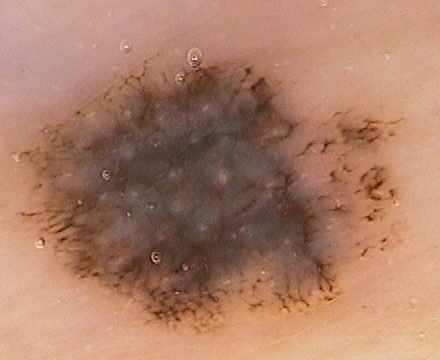
\includegraphics[width=0.2\textwidth, height= 0.12\textheight]{M1_PH2.png}}\hfill
  \subfloat[Dysplastic lesion]{
    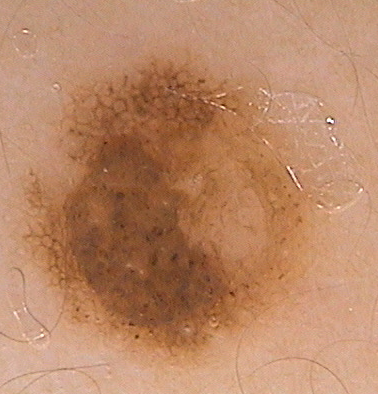
\includegraphics[width=0.2\textwidth, height= 0.12\textheight]{D1_PH2.png}}\hfill
  \subfloat[Benign lesion]{
    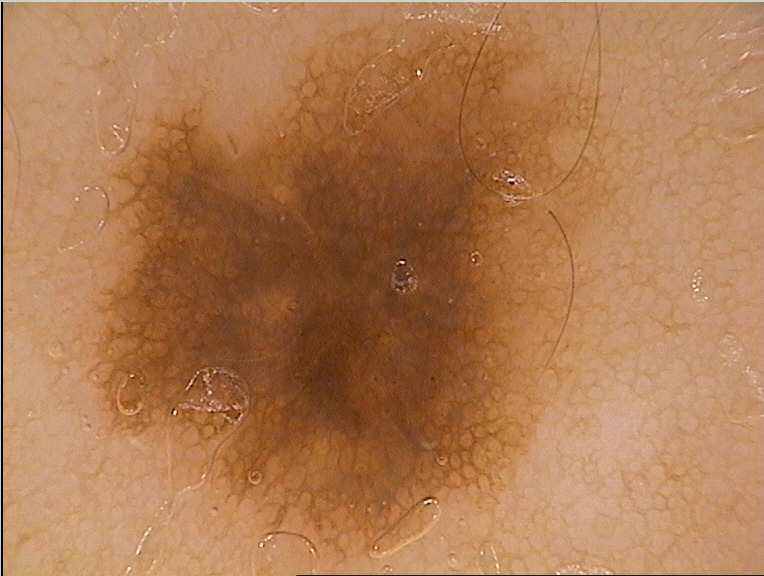
\includegraphics[width=0.2\textwidth, height= 0.12\textheight]{B1_PH2.png}}
  \hspace*{\fill}
  \caption{Samples of $PH^2$ dataset, representing melanoma, dysplastic and benign lesions, respectively}
  \label{fig:PH2samples}
\end{center}	
\end{figure*}
%Four images are discarded due to artifacts such as hair occlusions. 

Medical data are prone to such drawbacks due to the fact that the portion of diseased samples or patients is far lower than healthy cases.
Furthermore, the detection and classification of minority malignant cases are highly essential so that the \ac{se} of developed algorithms need to be maximized.
Consequently, the problem of imbalanced data is usually addressed by employing different techniques which do not vitiate the topology of the data.
Despite the fact that classification of malignant melanoma has been extensively studied~\cite{rastgoo2015automatic}, up to our knowledge, only few works tackled the issue implied by imbalanced dataset~\cite{barata2013two,celebi2007methodological}.
Barata~\emph{et al.} generate new synthetic samples by adding a Gaussian noise with fixed parameters to the samples belonging to the minority class~\cite{barata2013two}.
Celebi~\emph{et al.} and Capdehourat~\emph{et al.} over-sampled their dataset using \ac{smote}~\cite{chawla2002smote} to improve the \ac{se} of their algorithm~\cite{celebi2007methodological, capdehourat2009pigmented}.

This paper provides an insight to the specific problem of classification of imbalanced dataset for malenoma. 
To proceed, we review different techniques proposed by the machine learning community and compile a comprehensive quantitative evaluation. 
The rest of this paper is organized as follows: an overview of the classification framework designed to investigate data balancing techniques are presented through Sect.\,\ref{sec:mm} - Sect.\,\ref{sec:clas-val} while the balancing strategies are described in Sect.\,\ref{sec:met}.
A quantitative evaluation is discussed in Sect.\,\ref{sec:exp-res} followed by a concluding section.


% Some stuff that emac's colegues use
%%% Local Variables: 

%%% mode: latex
%%% TeX-master: "../../master"
%%% End: 

